\documentclass{beamer}
\usepackage{graphicx}
\usepackage{color}

\setlength{\parskip}{1em}

\newcommand{\clr}{\operatorname{clr}}
\newcommand{\N}{\operatorname{N}}
\newcommand{\cov}{\operatorname{cov}}
\newcommand{\var}{\operatorname{var}}

\DeclareMathOperator*{\argmax}{arg\,max}
\DeclareMathOperator{\tr}{tr}

\title{Covariance Properties and Graph Selection for High-Dimensional Compositional Data}
\author{Camden Lopez}
\date{June 6, 2017}

\begin{document}

\begin{frame}
\titlepage
\end{frame}

\begin{frame}
\frametitle{Outline}
\begin{itemize}
\item Compositional microbiome data
\item Graphical model and graphical lasso
\item Centered log-ratio transformation and SPIEC-EASI
\item Covariance properties and alternative covariances
\item Graph selection performance
\end{itemize}
\end{frame}

\begin{frame}
\frametitle{Compositional microbiome data}
16S amplicon sequencing:
\begin{enumerate}
\item Sample from environment
\item Extract DNA
\item Isolate and amplify 16S genes
\item Classify 16S genes by operational taxonomic unit (OTU)
\end{enumerate}
\begin{center}
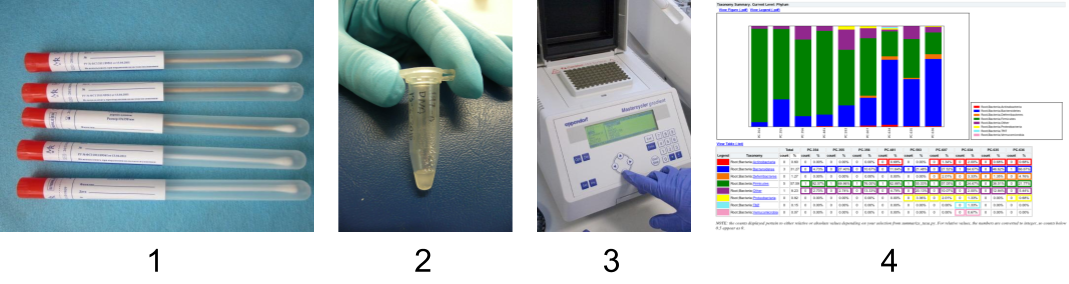
\includegraphics[width=300px]{figs/16s.png}
\end{center}
\end{frame}

\begin{frame}
\frametitle{Compositional microbiome data}
\begin{center}
\begin{tabular}{r|cccc}
Sample & OTU 1 & OTU 2 & $\dots$ & OTU $p$ \\
\hline
1 & $y_{11}$ & $y_{12}$ & $\dots$ & $y_{1p}$ \\
2 & $y_{21}$ & $y_{22}$ & $\dots$ & $y_{2p}$ \\
$\vdots$ & $\vdots$ & $\vdots$ & $\ddots$ & $\vdots$ \\
$n$ & $y_{n1}$ & $y_{n2}$ & $\dots$ & $y_{np}$
\end{tabular}
\end{center}

\begin{itemize}
\item $y_{ij} = $ \# sequences mapped to OTU $j$ in sample $i$
\item \textbf{Only relative proportions/ratios informative}
\end{itemize}
\end{frame}

\begin{frame}
\frametitle{Graphical model}
\textbf{Graphical model} representation of $V = (V_1, \dots, V_p)$
\begin{center}
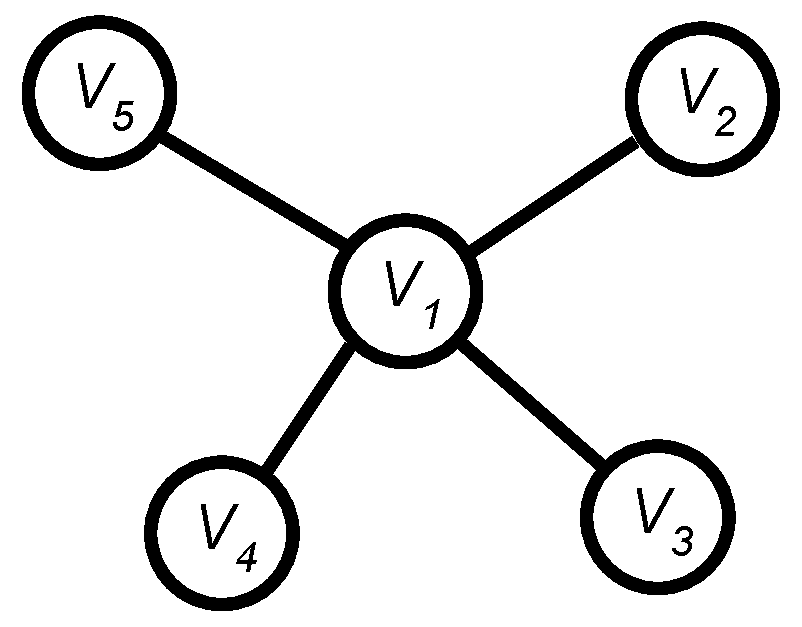
\includegraphics[width=100px]{figs/graph-model.pdf}
\end{center}
\begin{itemize}
\item \textbf{Nodes = variables, edges = conditional dependence}
\pause
\item Assuming $V \sim \N(\mu, \Sigma)$, $V_i$ and $V_j$ conditionally dependent if and only if $(\Sigma^{-1})_{ij} \ne 0$
\end{itemize}
\end{frame}

\begin{frame}
\frametitle{Goal of inference}
\textbf{Notation:}
\begin{align*}
W &= (W_1, \dots, W_p) = \text{absolute abundances of OTUs} \\
\Omega &= \cov(\log W)
\end{align*}
\pause
\textbf{Goal:}
\begin{itemize}
\item Infer conditional dependence relationships among $\log W_1, \dots, \log W_p$
\item Assuming $\log W \sim N(\,\cdot\,, \Omega)$, infer non-zero entries of $\Omega^{-1}$
\end{itemize}
\end{frame}

\begin{frame}
\frametitle{Centered log-ratio transformation}
\textbf{Centered log-ratio (clr) transformation:}
\begin{itemize}
\item Given sample $x = (x_1, \dots, x_p)$ with geometric mean $g(x) = (\prod_{i=1}^p x_i)^{\frac{1}{p}}$,
\end{itemize}
\pause
\begin{align*}
z = \clr(x) &= \left( \log \frac{x_1}{g(x)}, \dots, \log \frac{x_p}{g(x)} \right) \\
&= \left( \log x_1 - \frac{1}{p}\sum_{i=1}^p \log x_i, \dots, \log x_p - \frac{1}{p}\sum_{i=1}^p \log x_i \right)
\end{align*}
\pause
\textbf{Notation:}
\begin{itemize}
\item $\Gamma = \cov(\clr W)$
\end{itemize}
\end{frame}

\begin{frame}
\frametitle{SPIEC-EASI}
\textbf{SP}arse \textbf{I}nvers\textbf{E} \textbf{C}ovariance estimation for \textbf{E}cological \textbf{AS}sociation \textbf{I}nference (SPIEC-EASI)
\begin{itemize}
\item Estimate $\Gamma = \cov(\clr W)$ from compositional data
\item Infer non-zero entries of $\Omega^{-1}$ using $\hat{\Gamma}$, assuming $\Gamma \approx \Omega$
\end{itemize}
\pause
Graphical lasso estimate:
\begin{align*}
\widehat{\Omega^{-1}}_{glasso} &= \argmax_{\Omega^{-1}} \left[ \log \det(\Omega^{-1}) - \tr(\Omega^{-1} \widehat{\Omega}) - \lambda \lVert \Omega^{-1} \rVert_1 \right] \\
\widehat{\Omega^{-1}}_{SE} &= \argmax_{\Omega^{-1}} \left[ \log \det(\Omega^{-1}) - \tr(\Omega^{-1} \widehat{\Gamma}) - \lambda \lVert \Omega^{-1} \rVert_1 \right]
\end{align*}
\end{frame}

\begin{frame}
\frametitle{Covariance properties}
\textbf{Matrix form:}
\begin{align*}
\clr(W) &= \text{G} \log(W) \\
\text{G} &=
\begin{pmatrix}
1 - \frac{1}{p} & \dots & -\frac{1}{p} \\
\vdots & \ddots & \vdots \\
-\frac{1}{p} & \dots & 1 - \frac{1}{p}
\end{pmatrix} \\
\Rightarrow \Gamma &= \text{G} \Omega \text{G}
\end{align*}
\pause
\textbf{Entry form:}
\begin{equation*}
\gamma_{ij} = \omega_{ij} - \overline{\omega}_{i\cdot} - \overline{\omega}_{j\cdot} + \overline{\omega}_{\cdot\cdot}
\end{equation*}
\begin{itemize}
\item Rows (and columns) of $\Gamma$ sum to zero
\end{itemize}
\end{frame}

\begin{frame}
\frametitle{Covariance properties}
$\Gamma \approx \Omega$ when $-\overline{\omega}_{i\cdot} - \overline{\omega}_{j\cdot} + \overline{\omega}_{\cdot\cdot} \approx 0$
\begin{itemize}
\item $\Omega$ row averages all small (``sparse" covariances)
\item Larger $p$ helps if $\Omega$ row sums increase slower than $p$
\item \textbf{Small ``compositional effect"}
\end{itemize}
\pause
$\Gamma \not\approx \Omega$
\begin{itemize}
\item Some or all $\Omega$ row averages large
\item Many positive correlations, or some extremely large variances
\item \textbf{Large ``compositional effect"}
\end{itemize}
\end{frame}

\begin{frame}
\frametitle{Alternative covariances}
\textbf{Given $\Gamma$, what could $\Omega$ be?}
\begin{itemize}
\item $\Gamma$ has $p$ fewer free parameters than $\Omega$: \\$\frac{1}{2}p(p-1)$ vs. $\frac{1}{2}p(p+1)$
\item Each $\Gamma$ associated with a $p$ dimensional space of possible $\Omega$s
\end{itemize}
\pause
Solving for $\Omega$, given $\Gamma$ and choosing $\omega_{11}, \dots, \omega_{pp}$:
\begin{equation*}
\omega_{ij} = \gamma_{ij} + \frac{1}{2}(\omega_{ii} - \gamma_{ii} + \omega_{jj} - \gamma_{jj})
\end{equation*}
\pause
\begin{itemize}
\item Check that $\Omega$ is \textbf{positive definite} (valid covariance)
\end{itemize}
\end{frame}

\begin{frame}
\frametitle{Alternative covariances: $p = 2$}
Can analyze and visualize $p = 2$ case:
\begin{itemize}
\item $\Omega$ positive definite iff $\det(\Omega) > 0$
\item Can find where $\omega_{12} < 0$, $\omega_{12} = 0$, or $\omega_{12} > 0$
\end{itemize}
\pause
\begin{center}
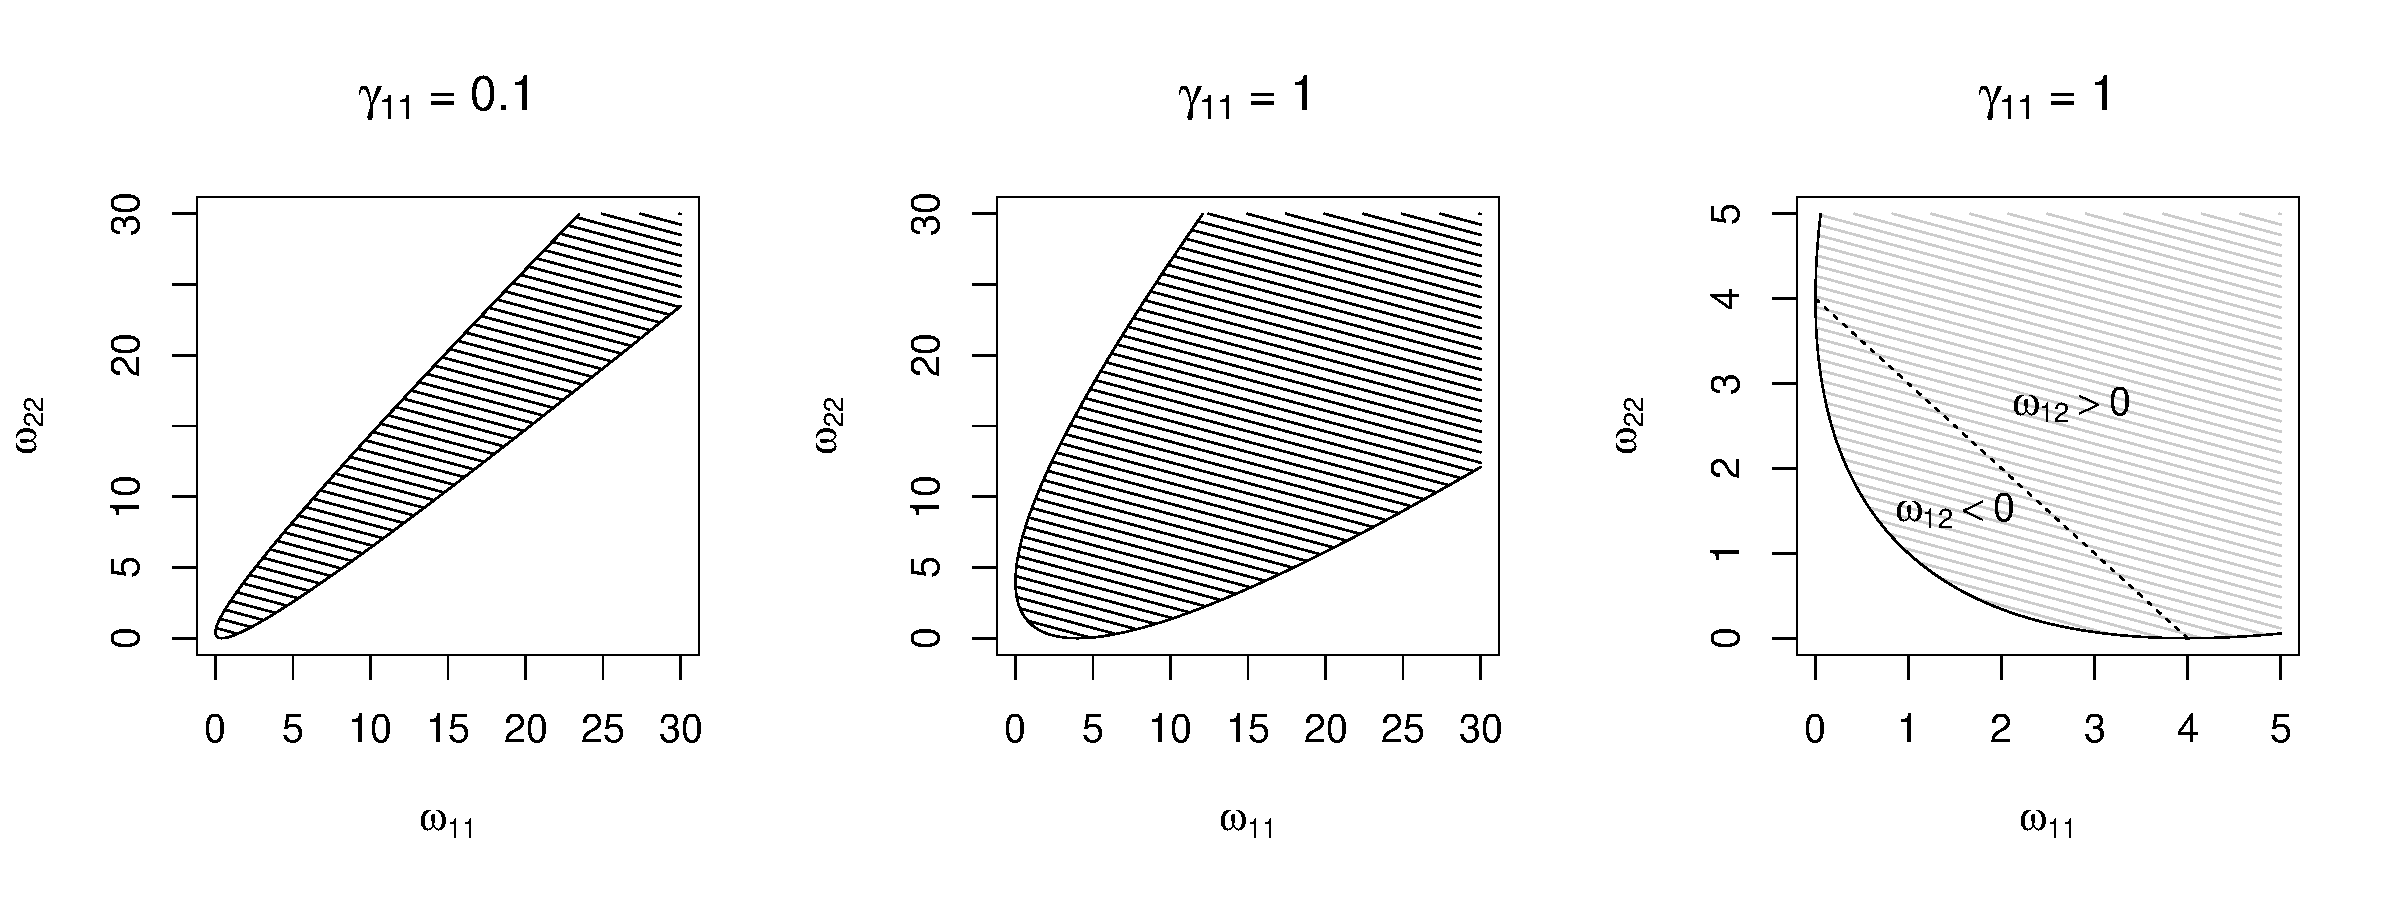
\includegraphics[width=300px]{figs/regions-2.pdf}
\end{center}
\end{frame}

\begin{frame}
\frametitle{Alternative covariances: $p = 2$}
Example:
\begin{itemize}
\item (a) clr abundances
\item (b) log abundances with $\omega_{11} = 0.7$, $\omega_{22} = 4.3$, $\omega_{12} = 1.7$
\item (c) log abundances with $\omega_{11} = 0.7$, $\omega_{22} = 0.3$, $\omega_{12} = -0.3$
\end{itemize}
\begin{center}
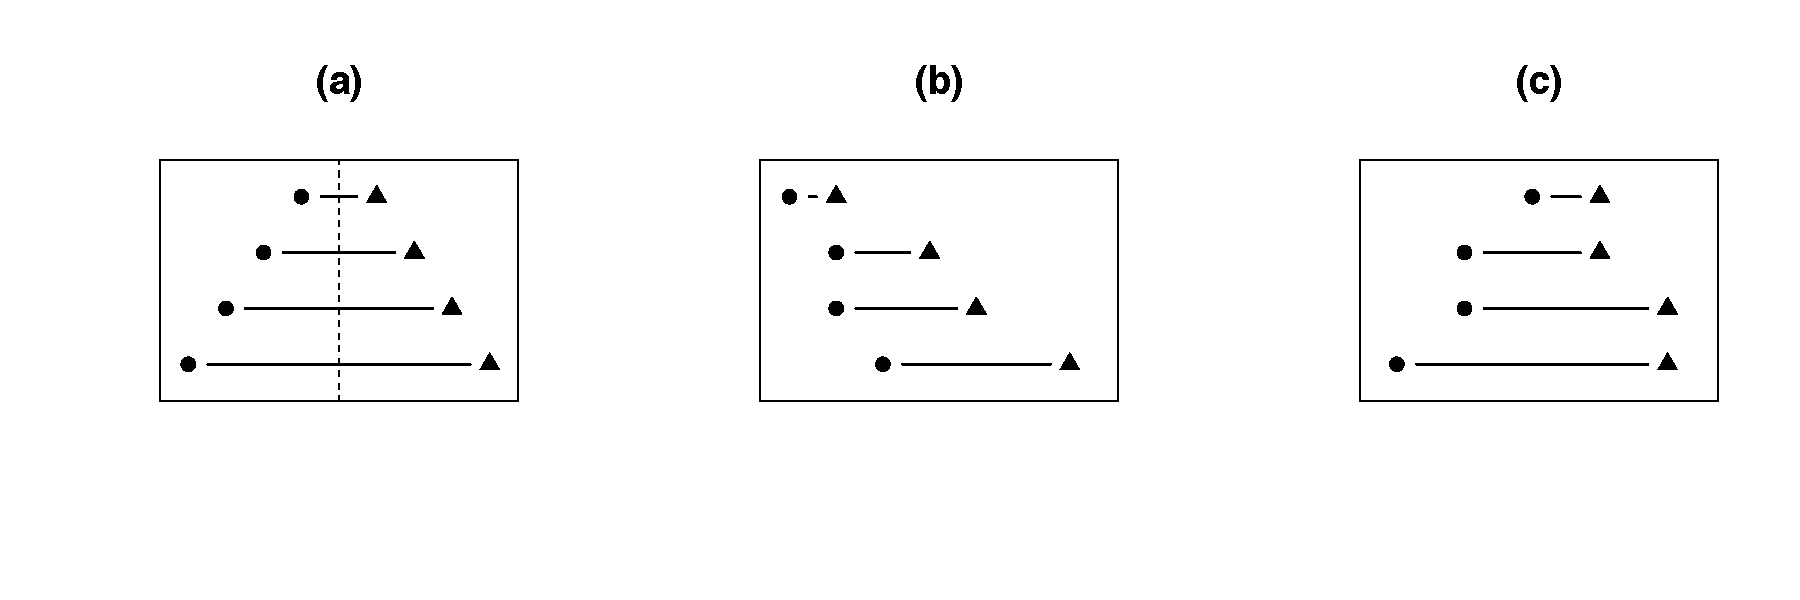
\includegraphics[width=300px]{figs/example-2.pdf}
\end{center}
\end{frame}

\begin{frame}
\frametitle{Alternative covariances: larger $p$}
More complicated to analyze\textellipsis
\begin{itemize}
\item Investigated several examples by trial-and-error
\end{itemize}
\pause
Example: $\Gamma$ corresponding to $\Omega$ used in $p = 64$ simulations
\begin{itemize}
\item Similar \textbf{limits on potential variances} $\omega_{11}, \dots, \omega_{pp}$
\begin{center}
\begin{tabular}{r|rrrrrr}
& $\omega_{11}$ & $\omega_{22}$ & $\omega_{33}$ & $\omega_{44}$ & $\omega_{55}$ & $\dots$ \\
\hline
min & 0.22 & 0.30 & 0.18 & 0.22 & 0.18 & $\dots$ \\
max & 0.39 & 0.47 & 0.36 & 0.40 & 0.36 & $\dots$
\end{tabular}
\end{center}
\item Unconditional relationships ($\Omega$ entries) and conditional relationships ($\Omega^{-1}$) can \textbf{vary widely}
\end{itemize}
\end{frame}

\begin{frame}
\frametitle{Alternative covariances: larger $p$}
Partial correlations
\begin{itemize}
\item Indicate signs and strengths of conditional relationships
\item {\color{blue} Blue} = positive, {\color{red} red} = negative partial correlation
\pause
\item (a) $\omega_{ii} = \gamma_{ii} + 10^{-4}$ for all $i$
\item (b) $\omega_{ii} = \gamma_{ii} + 10^{-3}$ for all $i$
\item (c) $\omega_{ii} = \gamma_{ii} + 10^{-2}$ for all $i$
\item (d) Small $\omega_{ii}$ in first cluster, others equal to values in initial $\Omega$
\item (e) All $\omega_{ii}$ equal to values in initial $\Omega$
\item (d) Large $\omega_{ii}$ in first cluster, others equal to values in initial $\Omega$
\end{itemize}
\end{frame}

\begin{frame}
\frametitle{Alternative covariances: larger $p$}
\begin{center}
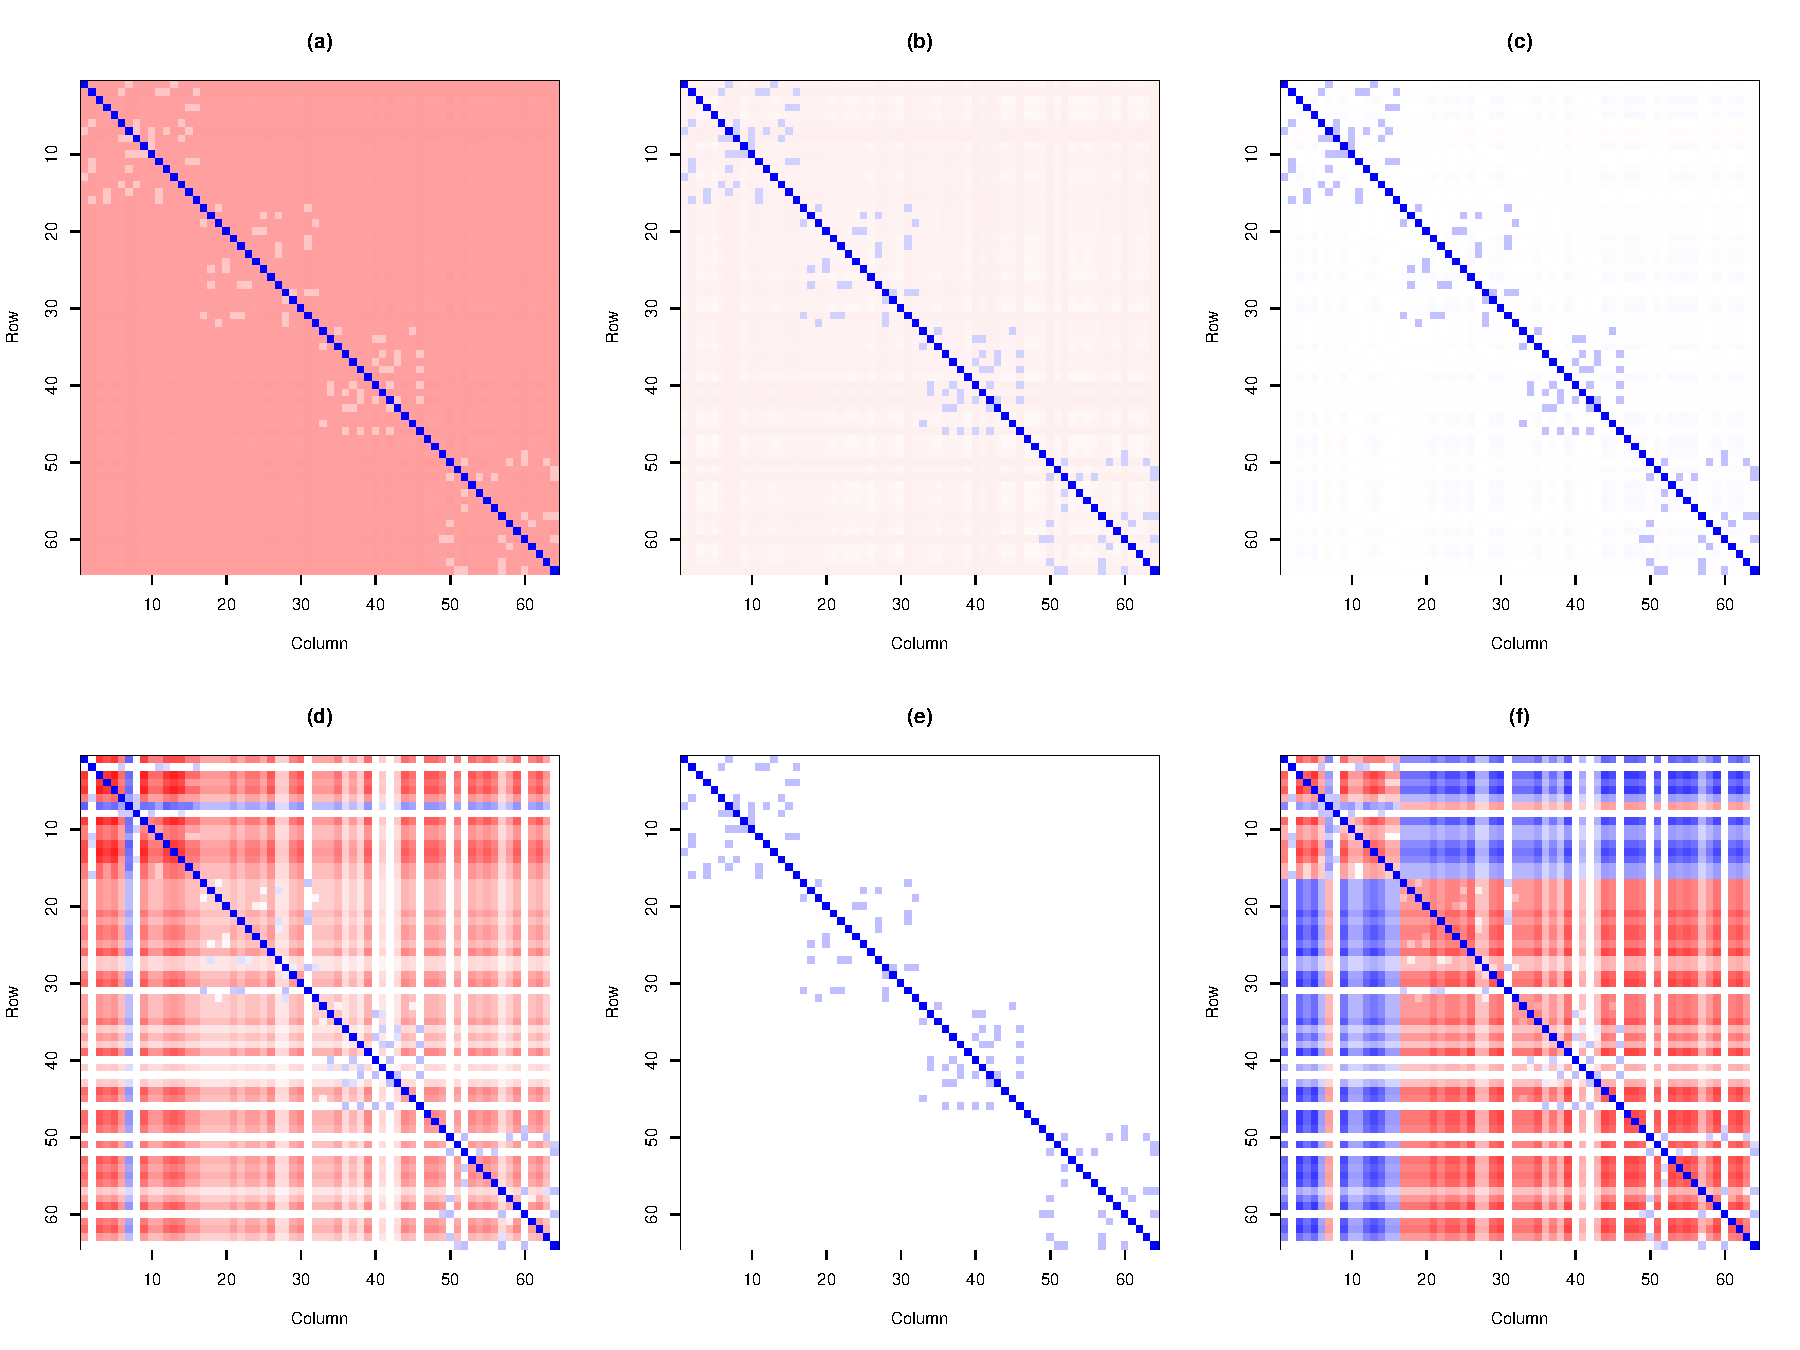
\includegraphics[width=275px]{figs/pcor.pdf}
\end{center}
\end{frame}

\begin{frame}
\frametitle{Performance: simulation setup}
\textbf{How well does it work in ideal settings?}

\begin{itemize}
\item Three sparse graph structures ($p-1$ edges in each)
\item Graph $\rightarrow \Omega^{-1}$ (p. cor. $\pm 0.25$) $\rightarrow \Omega$
\item $\log W \sim \N(0, \Omega)$
\end{itemize}
\begin{center}
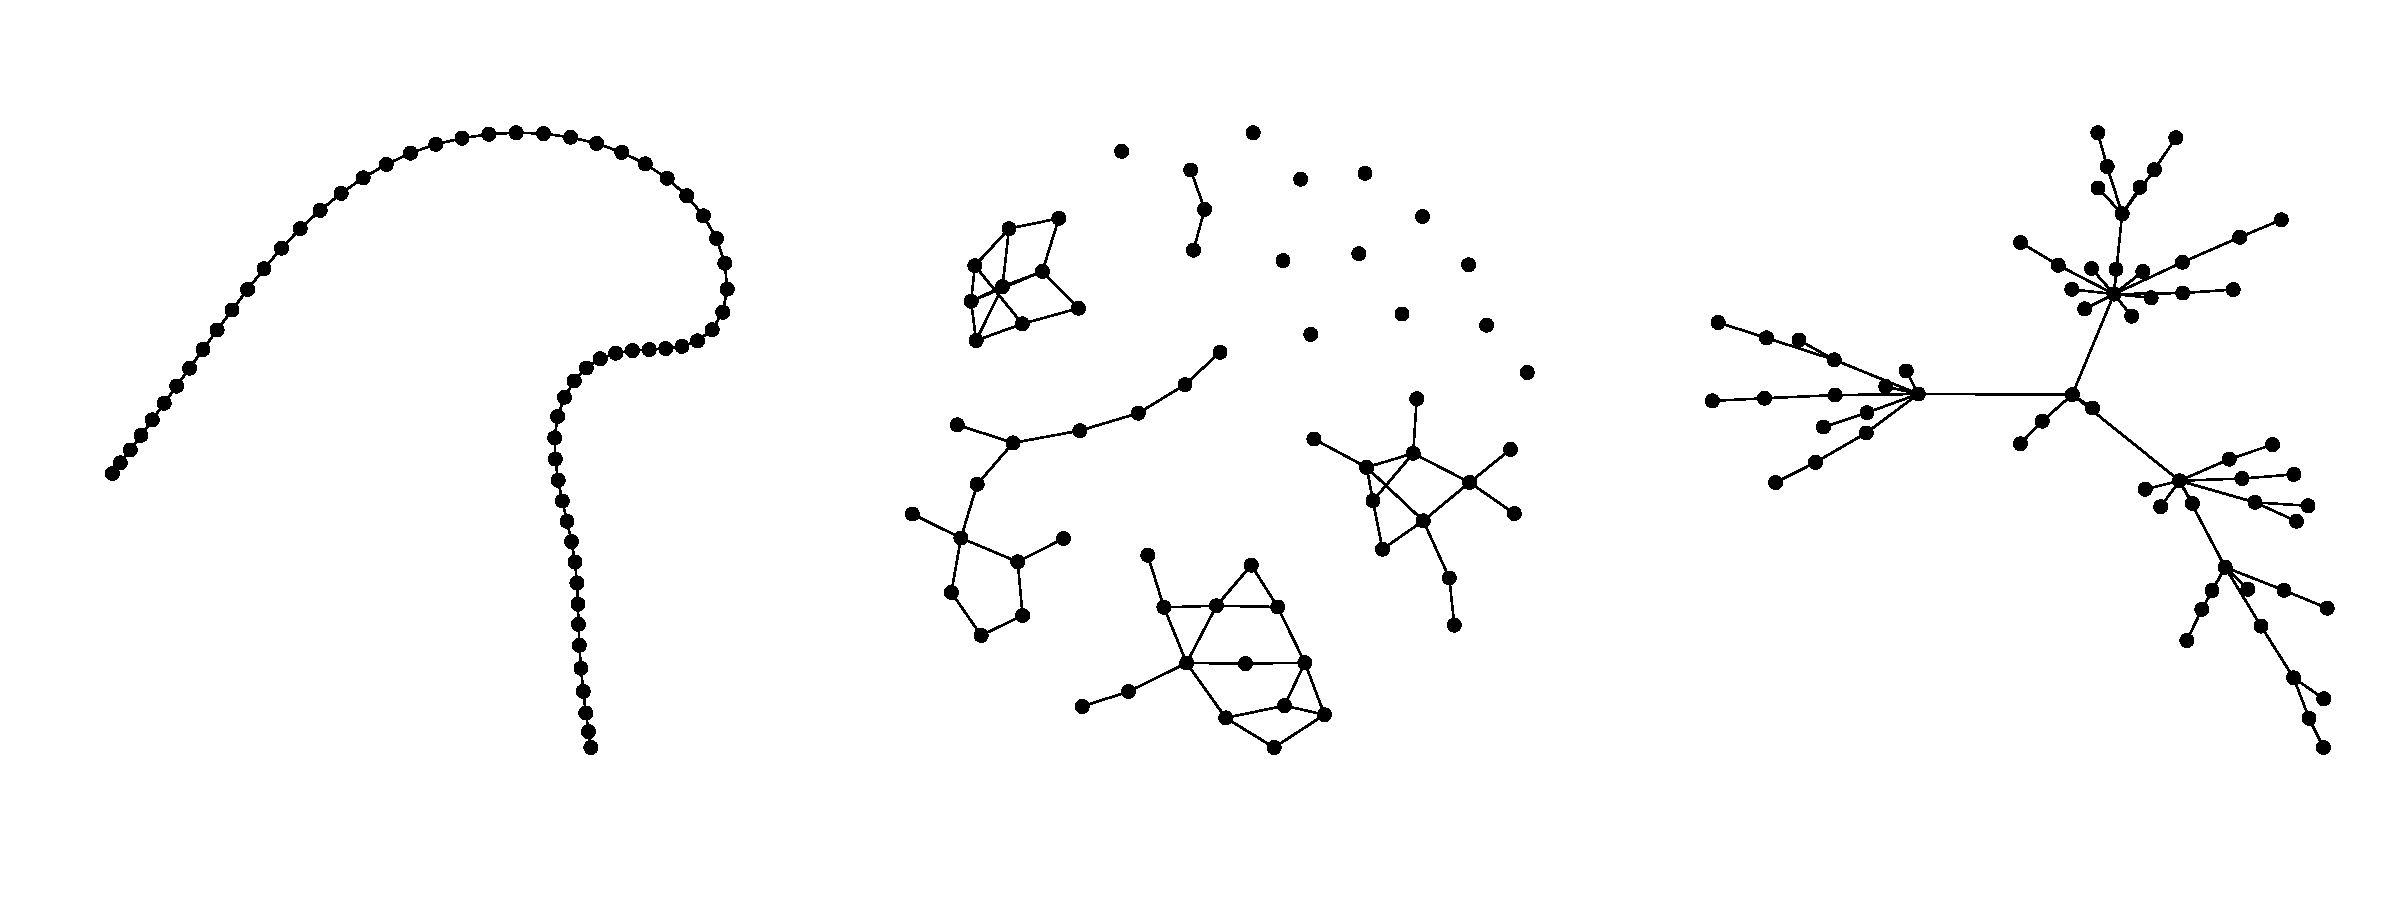
\includegraphics[width=250px]{figs/graphs-64.pdf}
\end{center}
\end{frame}

\begin{frame}
\frametitle{Performance: simulation setup}
\textbf{Performance metric:}
\begin{itemize}
\item Area under precision-recall curve (AUPR)
\item Points on curve $\leftrightarrow$ graphical lasso solutions for $\lambda_{min} < \dots < \lambda_{max}$
\item Using both log and clr data for comparison
\end{itemize}
\begin{align*}
\text{Recall} &= \frac{\text{\# correctly selected edges}}{\text{\# edges in true graph}} \\
\text{Precision} &= \frac{\text{\# correctly selected edges}}{\text{\# edges selected}}
\end{align*}
\end{frame}

\begin{frame}
\frametitle{Performance: simulation setup}
\textbf{Precision-recall curves (example):}
\begin{center}
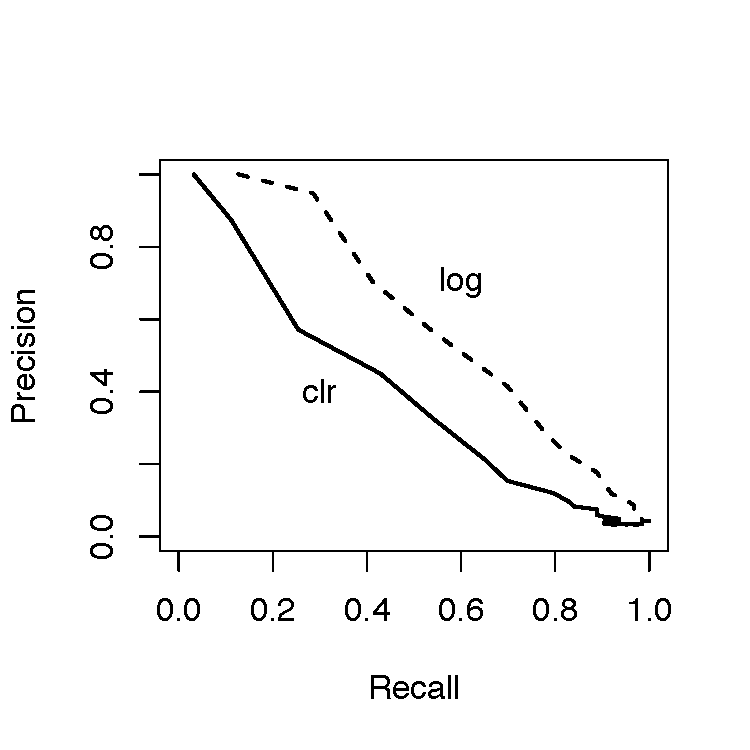
\includegraphics[width=200px]{figs/pr-curve.pdf}
\end{center}
\end{frame}

\begin{frame}
\frametitle{Performance: $p = 64$}
\begin{center}
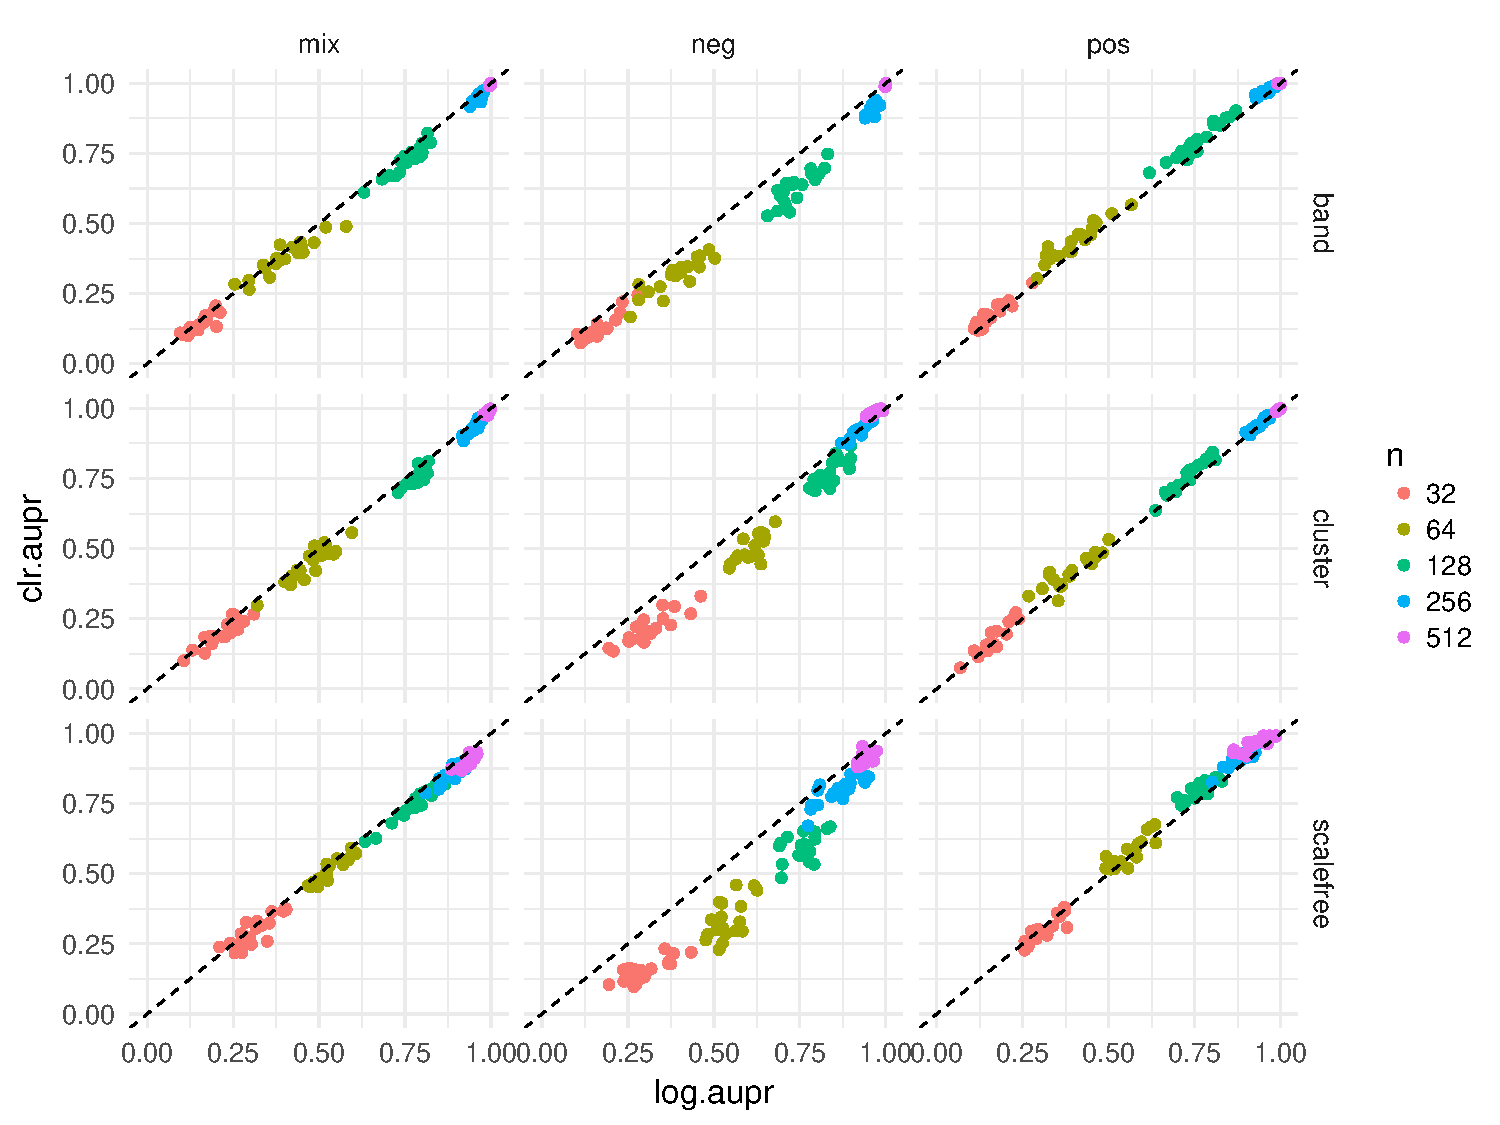
\includegraphics[width=300px]{figs/glasso-64.pdf}
\end{center}
\end{frame}

\begin{frame}
\frametitle{Performance: $p = 256$}
\begin{center}
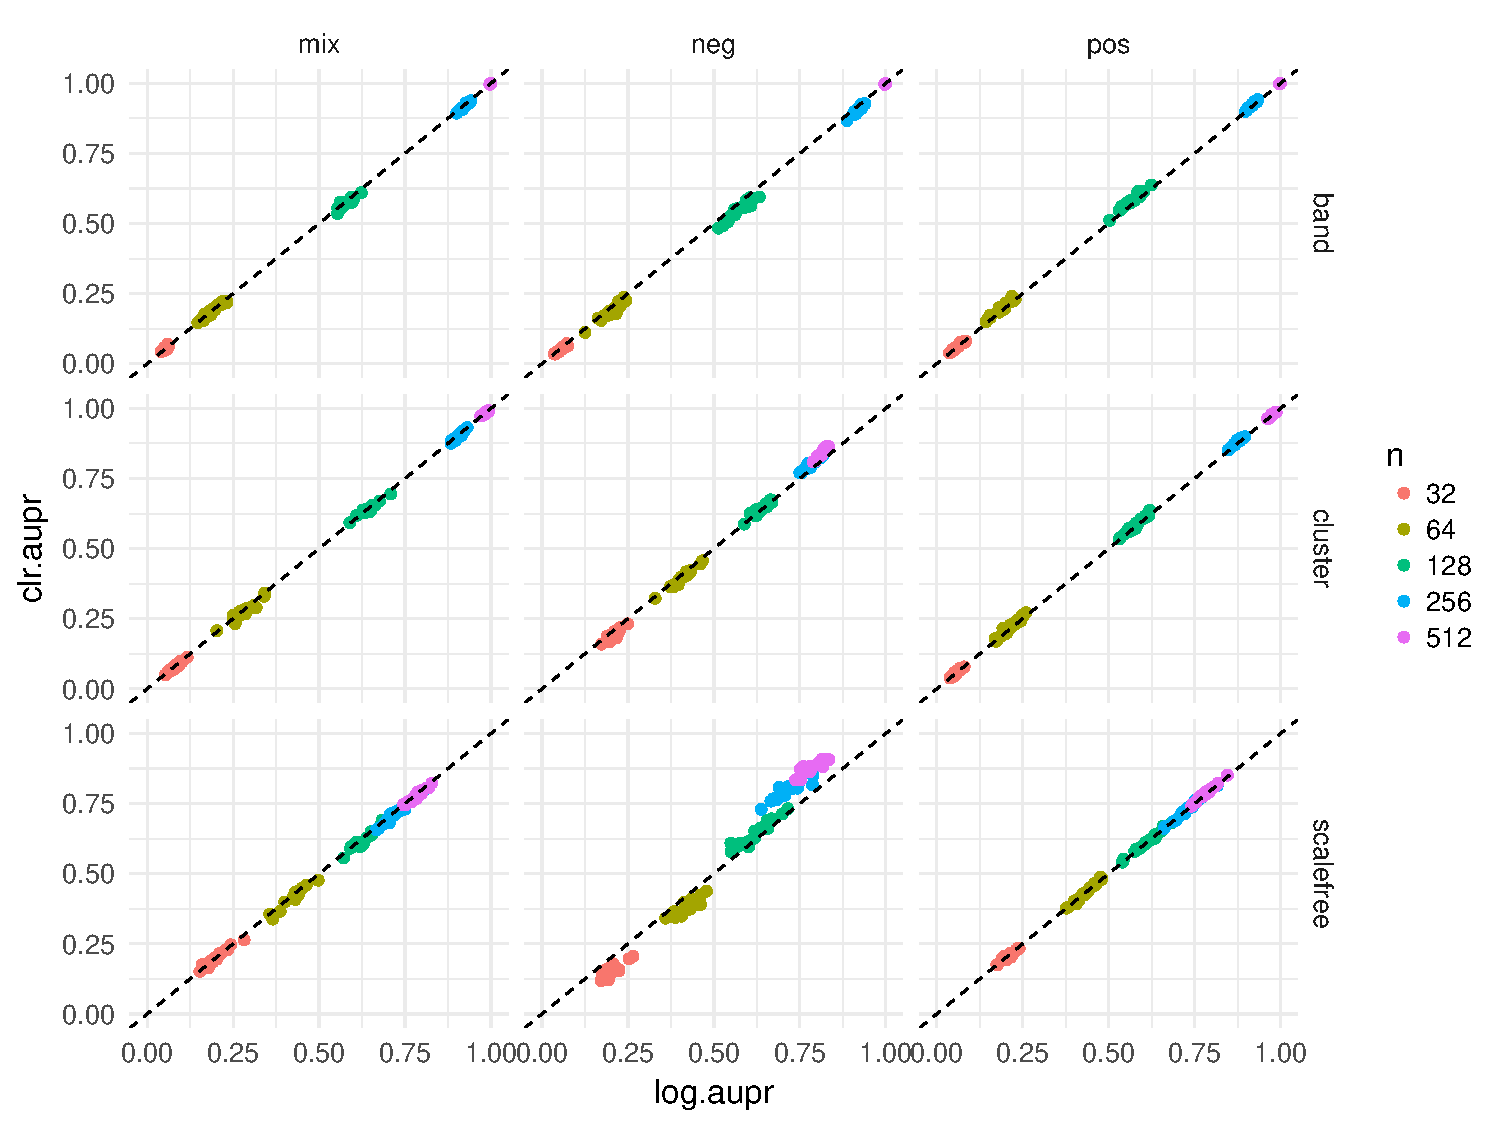
\includegraphics[width=300px]{figs/glasso-256.pdf}
\end{center}
\end{frame}

\begin{frame}
\frametitle{Performance: large compositional effect}
\textbf{What if there's a large compositional effect?}
\begin{itemize}
\item Same setting as $p=64$ simulations, but $\omega_{11}$ 400 times larger
\item (---) = clr, (- - -) = log
\end{itemize}
\begin{center}
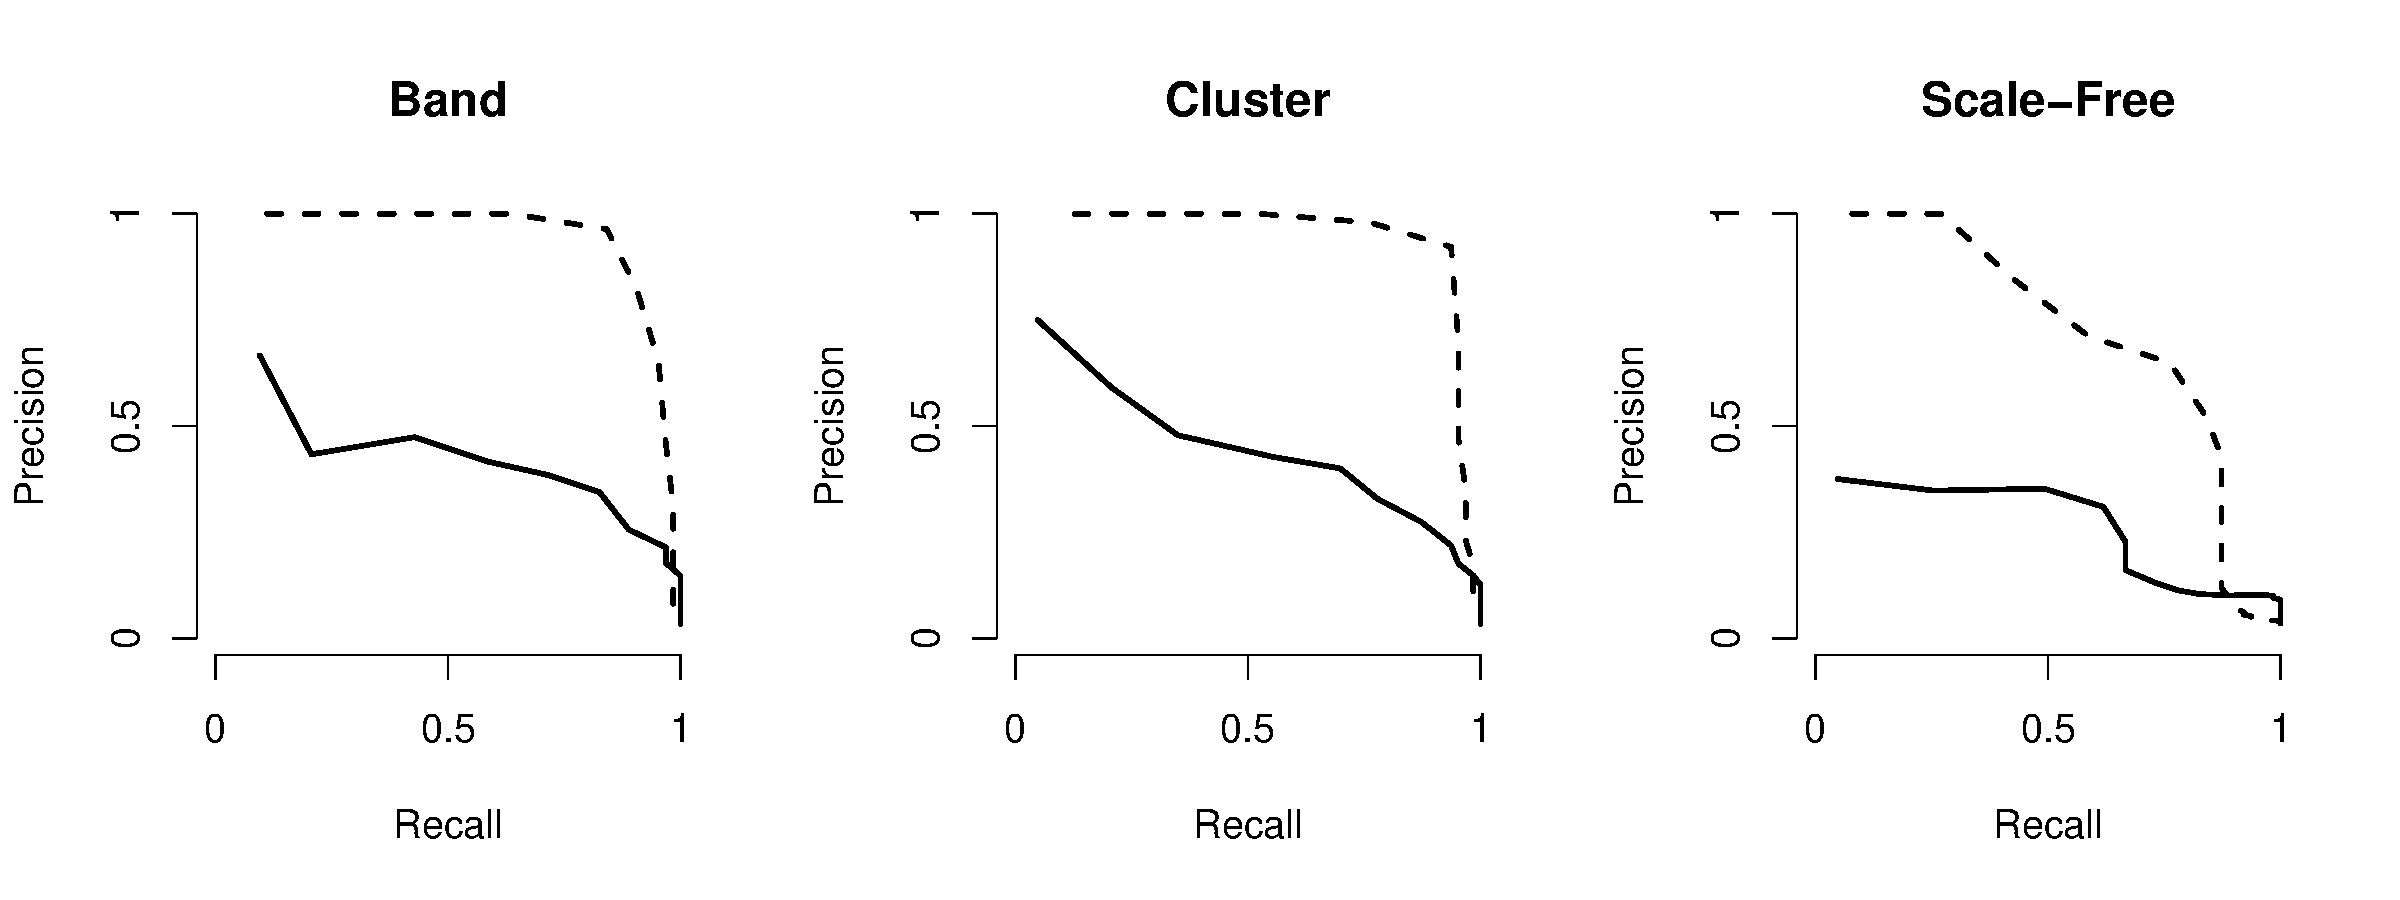
\includegraphics[width=300px]{figs/var-dom-pr.pdf}
\end{center}
\end{frame}

\begin{frame}
\frametitle{Performance: large compositional effect}
\textbf{Spurious edges due to compositional effect:}
\begin{itemize}
\item Truth (left) vs. log data (center) vs. clr data (right)
\end{itemize}
\begin{center}
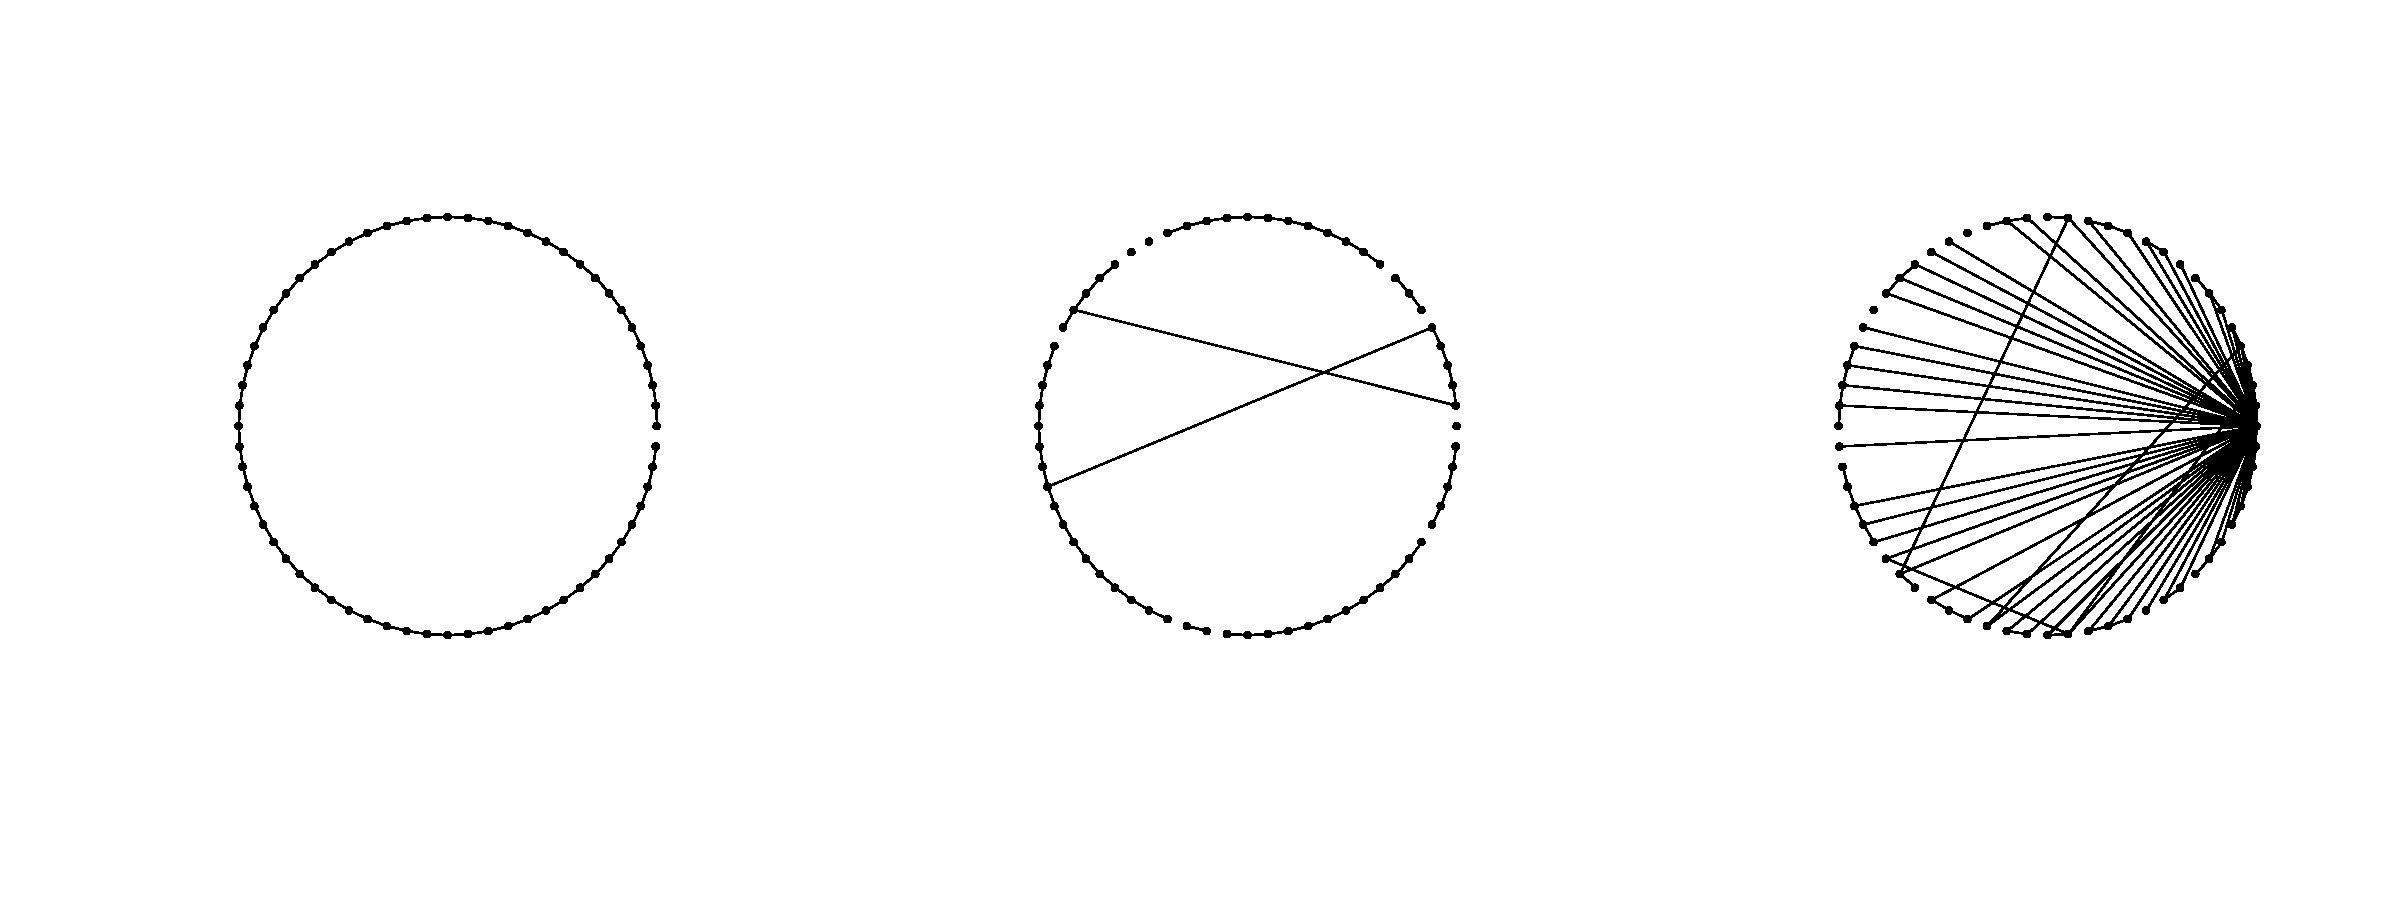
\includegraphics[width=250px]{figs/var-dom-band.pdf} \\
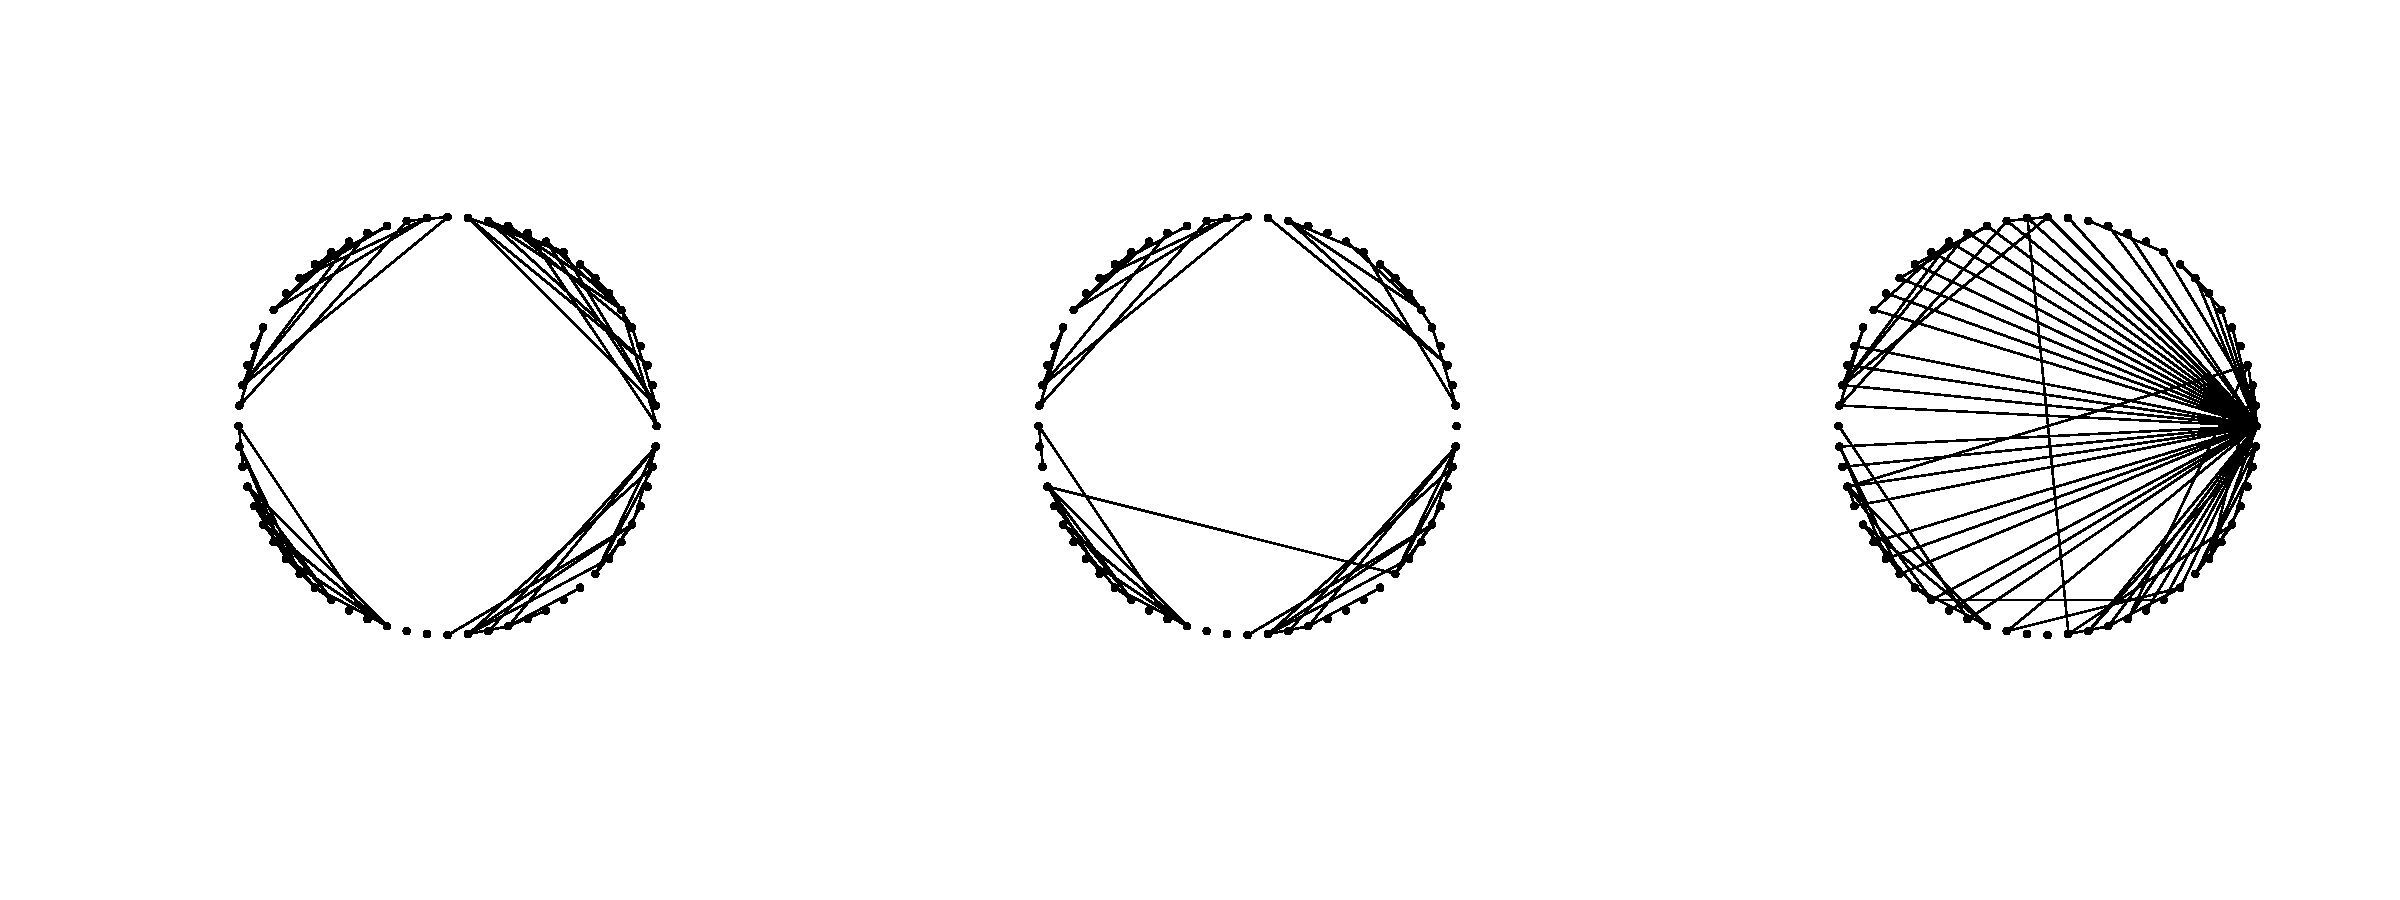
\includegraphics[width=250px]{figs/var-dom-cluster.pdf}
\end{center}
\end{frame}

\begin{frame}
\frametitle{Conclusion}
\textbf{Graph selection:}
\begin{itemize}
\item Performs well when there isn't a large compositional effect
\item Otherwise can select spurious edges
\end{itemize}

\textbf{Limitation of compositional data:}
\begin{itemize}
\item Covariances of clr data could correspond to a variety of log abundance covariances
\item Variety of possible conditional and unconditional relationships
\end{itemize}
\end{frame}

\begin{frame}
\frametitle{References}
Aitchison, J. (1986). \textit{The Statistical Analysis of Compositional Data}. Chapman and Hall, London, UK.

Friedman, J., Hastie, T., and Tibshirani, R. (2008). Sparse inverse covariance estimation with the graphical lasso. \textit{Biostatistics} 9, 432--441.

Kurtz., Z. D., M{\"u}ller, C. L., Miraldi, E. R., Littman, D. R., Blaser, M. J., and Bonneau, R. A. (2015). Sparse and compositionally robust inference of microbial ecological networks. \textit{PLoS Computational Biology} 11, e1004226.
\end{frame}
\end{document}